% =====================================================================
\chapter{Study 2: Downstream Judgements of Image Search Results}\label{ch:study2}
% =====================================================================

% \begin{plan}[Chapter plan --- Study 2 (RQ2, Aim 4)]
% \pages{8 pages.} \textbf{Order of the argument:} (1) measurement quality;
% (2) CALM robustness --- the strongest result, replicated across architectures;
% (3) \emph{why} it collapses (anchor following); (4) deviation from the human
% baseline, with the definition and sign decisions D1--D2 settled first; (5) the
% person vs non-person dissociation; (6) link back to the SIGIR findings.
% \citeplan{otterbacher2018sigir,ye2025justice,zheng2023judging,wang2024fair,chen2024mllmjudge,zheng2024robust,field2007bootstrapping}
% \end{plan}

% ---------------------------------------------------------------------
\section{Study overview}\label{sec:s2-aims}\label{sec:s2-quality}

Study 2 examines whether the inventory responses reported in \cref{ch:study1}
correspond with judgements of image search results. Five models evaluated
nine images for each of ten queries from Otterbacher et al.\
\cite{otterbacher2018sigir}, under original and reversed scales and with
or without the image. Human participants rated the corresponding grids,
so the model ratings are averaged by query for the human comparison.

The analysis tests three expectations: robustness should remain similar
between conditions if visual evidence has little influence, ratings resembling
the low-ASI group should have deviations near zero, and differences specific
to person queries should be reduced on the non-person control. These
comparisons address the evaluated protocols, rather than isolating components
within the models.

Mean captured mass over the rating digits is $0.9944$ for Llama-11B,
$0.9971$ for Qwen-2B, $0.9978$ for Llama-90B, $0.9993$ for Qwen-7B and
$0.9996$ for Qwen-72B. Coverage is therefore high across all models, unlike
the binary probe, although high coverage alone does not establish valid
or consistent judgements. The results below first examine scale reversal,
then compare ratings with the human baseline.

\section{Robustness under scale reversal}\label{sec:s2-calm}

Scale reversal exchanges the meanings of the endpoints while retaining the
underlying judgement: a raw rating $r$ should become $8-r$.
\Cref{tab:s2-rr} reports agreement after normalisation, with the primary
comparison shown in \cref{fig:s2-rr}. Three observations summarise the result:

\begin{enumerate}[leftmargin=*,itemsep=0.5em]
\item At $\tau=0.5$, Llama-90B and Qwen-72B each achieve robustness of
$0.900$ without an image, falling to $0.044$ and $0.156$ in the image
condition. This corresponds to agreement on four of 90 image pairs for
Llama-90B and 14 of 90 for Qwen-72B, compared with nine of ten distinct
query pairs without images. Their differences are $\dRR=-0.856$ and
$-0.744$, with 95\% intervals of $[-0.98,-0.66]$ and $[-0.98,-0.50]$, respectively.
Both intervals exclude zero, so the expectation of similar robustness
between conditions is unsupported for the two largest models. The separation
also persists at the other two tolerances shown in the table.

\item The smaller models have low robustness in both conditions, giving
small differences against an already unreliable baseline. Qwen-2B changes
from $0.200$ to $0.189$, Qwen-7B from $0.200$ to $0.156$, and Llama-11B
from $0.000$ to $0.022$. Their near-zero differences consequently should
not be interpreted as evidence of stable ratings.

\item The conditions differ in referent wording as well as image presence,
using ``a typical result'' without an image and ``this image result''
with one. The comparison therefore establishes lower robustness in the
image condition for the two largest models, without identifying a causal
effect of visual input alone.
\end{enumerate}

Intervals use $B=10{,}000$ bootstrap resamples of the ten queries, following
\cref{sec:framework-calm}. The text-only condition contains 90 recorded
pairs but only ten distinct query-level pairs, each repeated for nine images;
resampling rows would incorrectly treat those repetitions as independent
information.

\begin{table}[htbp]\centering\small
\begin{tabular}{@{}lccccc@{}}
\toprule
& \multicolumn{3}{c}{$\RR_{\text{vision}}(\tau)$ / $\RR_{\text{text}}(\tau)$} & $\dRR(0.5)$ & 95\% CI \\
\cmidrule(lr){2-4}
Model & $\tau=0.25$ & $\tau=0.5$ & $\tau=1$ & & \\
\midrule
Qwen-2B & 0.111 / 0.20 & 0.189 / 0.20 & 0.400 / 0.70 & $-0.011$ & $[-0.30,+0.27]$ \\
Qwen-7B & 0.022 / 0.10 & 0.156 / 0.20 & 0.267 / 0.60 & $-0.044$ & $[-0.38,+0.22]$ \\
Llama-11B & 0.022 / 0.00 & 0.022 / 0.00 & 0.078 / 0.00 & $+0.022$ & $[+0.00,+0.06]$ \\
Qwen-72B & 0.089 / 0.80 & 0.156 / 0.90 & 0.267 / 1.00 & $-0.744$ & $[-0.98,-0.50]$ \\
Llama-90B & 0.000 / 0.90 & 0.044 / 0.90 & 0.300 / 1.00 & $-0.856$ & $[-0.98,-0.66]$ \\
\bottomrule
\end{tabular}
\caption{Robustness rate under CALM scale reversal. Vision: 90 pairs; text-only:
90 rows but 10 distinct pairs. Interval: cluster bootstrap over the 10 queries
($B=10{,}000$), resampling queries rather than rows.}
\label{tab:s2-rr}\label{tab:app-rr-full}
\end{table}
\begin{figure}[htbp]\centering
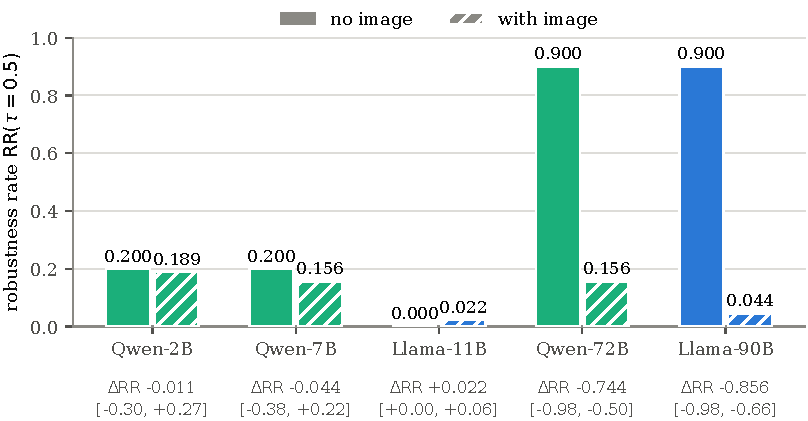
\includegraphics[width=\linewidth]{s2-rr.pdf}
\caption{Robustness rate under scale reversal at $\tau=0.5$, with and without the
image. Values beneath each model are $\dRR$ with a percentile interval from a
cluster bootstrap over the ten queries, $B=10{,}000$, which resamples queries
rather than rows.}
\label{fig:s2-rr}
\end{figure}

\subsection{Scale anchors and paired agreement}\label{sec:s2-anchor}

The raw-rating analysis in \cref{fig:s2-anchor} complements robustness by
examining the relationship between the two scale orientations.
Exact transformation requires $y=8-x$, including both slope $-1$ and
intercept 8, so a fitted slope alone cannot establish correct anchor use.
The mean raw ratings are retained in \cref{tab:s2-anchor}.

Without images, the fitted slopes are $-0.97$ for Llama-90B and $-1.03$
for Qwen-72B, changing to $-0.87$ and $-0.67$ with images.
The negative slopes preserve the overall direction of scale reversal, but
the ratings are displaced from the required transformation. With images,
Llama-90B's mean reversed rating is $4.64$ rather than the $3.21$ required
by its mean original rating; Qwen-72B gives $4.19$ rather than $2.50$.
These offsets of $1.43$ and $1.69$ scale points show how a negative
relationship can coexist with poor agreement between paired judgements.

The smaller models also depart from the ideal transformation, with Qwen-2B
giving a slope of $+0.79$ in both conditions and Qwen-7B changing from
$-0.06$ to $+0.74$. These diagnostics describe the observed ratings without
identifying how the models process the scale instructions.

\clearpage
\begin{figure}[htbp]\centering
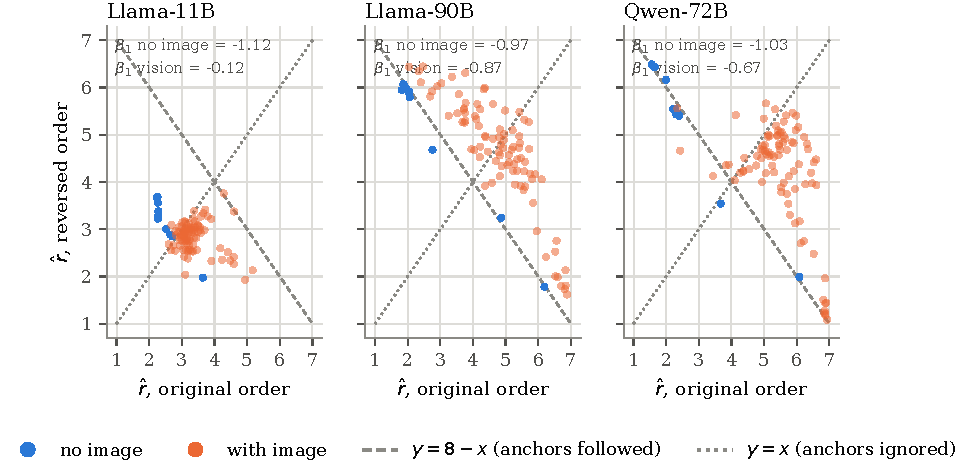
\includegraphics[width=\linewidth]{s2-anchor.pdf}
\caption{Expected rating under the reversed scale against the expected rating under the
original scale, one point per pair. The five panels compare both image
conditions with the ideal anchor
transformation $y=8-x$. The two largest models follow this relationship
closely without an image. With an image, pairwise agreement weakens;
Llama-90B retains a negative fitted slope, so its robustness loss does not
indicate a reversal to a positive relationship.}
\label{fig:s2-anchor}
\end{figure}

\section{Comparison with human judgements}\label{sec:s2-deviation}

The primary deviation $\dm$ compares original-order model ratings with the
mean grid ratings of participants at or below the median total ASI score
(\cref{eq:deltam}). A negative value indicates lower perceived objectivity
than this baseline, while a positive value indicates higher perceived
objectivity. This comparison does not establish whether a model is more
or less sexist than the human group.

\Cref{tab:s2-deltam} shows that Qwen-72B rates the results slightly above
the baseline ($+0.216$), while Qwen-7B is closest in absolute terms
($-0.066$). The remaining deviations are $-0.491$ for Llama-90B, $-0.834$
for Qwen-2B and $-1.920$ for Llama-11B. These positions require caution
because the models' ratings are unstable under scale reversal.

The order-averaged values illustrate the risk of combining the orientations:
Llama-90B's $-1.203$ is only $0.077$ from the anchor-insensitivity null
of $-1.280$. Proximity does not prove anchor insensitivity, but makes the
order-averaged result difficult to interpret independently of that response
pattern. The original order is therefore primary, with the alternative
values retained as sensitivity comparisons.

Across five models, the correlation between aggregate inventory scores and
signed original-order deviations is $\rho=-0.70$. Models with higher
aggregate scores therefore tend to rate the results as less objective relative
to the human baseline, differing in direction from the original human
association. An exact two-sided permutation calculation gives $p=0.233$,
with 28 of 120 rank permutations producing an equally or more extreme
correlation. This calculation assumes exchangeable model pairings, while
variants within each family are related; the comparison therefore remains
descriptive. Its interpretation is also limited by the small sample and
the aggregate score's sensitivity to agreement tendencies.

The analysis above uses the low-ASI group as the single reference.
\Cref{sec:s2-subscale} repeats the split on each ASI subscale and reports
the comparison with the high scoring groups.

\begin{table}[htbp]\centering\small
\begin{tabularx}{\linewidth}{@{}>{\raggedright\arraybackslash}Xccccc@{}}
\toprule
$\dm$ variant & Qwen-2B & Qwen-7B & Llama-11B & Qwen-72B & Llama-90B \\
\midrule
Original order only (\cref{eq:deltam}) & $-0.834$ & $-0.066$ & $-1.920$ & $+0.216$ & $-0.491$ \\
Reversed order only & $-2.014$ & $-1.697$ & $-0.123$ & $-1.467$ & $-1.916$ \\
Order-averaged & $-1.424$ & $-0.881$ & $-1.022$ & $-0.625$ & $-1.203$ \\
Anchor-insensitivity null (\cref{prop:null}) & $-1.280$ & $-1.280$ & $-1.280$ & $-1.280$ & $-1.280$ \\
\bottomrule
\end{tabularx}
\caption{Extrinsic deviation from the SIGIR 2018 low-ASI baseline under the
candidate definitions (vision rows, 90 per order).}
\label{tab:s2-deltam}
\end{table}

\subsection{Subscale splits of the human baseline}\label{sec:s2-subscale}

The deviation above splits the participants at the median total ASI score,
while the association reported by Otterbacher et al.\
\cite{otterbacher2018sigir} concerned the benevolent subscale. The released
data stores a benevolent and a hostile score for each participant, so the
split can be repeated on each subscale without rescoring the items.
\Cref{tab:s2-human-splits} reports the three splits.

Both subscale splits separate the groups more widely than the total score.
The high minus low contrast is $+0.352$ on the benevolent subscale and
$+0.333$ on the hostile subscale, against $+0.179$ on the total score. These
two contrasts are close to each other and the two scores correlate at
$r=0.587$, so neither contrast on its own identifies which subscale carries
the association. Entering both as standardised predictors of each
participant's mean objectivity rating separates them: the benevolent
coefficient is $+0.168$ ($p=0.039$) while the hostile coefficient falls to
$+0.004$ ($p=0.957$), and $R^{2}$ stays at $0.024$, the value reached by the
benevolent predictor alone. Among these participants the association is
therefore specific to the benevolent subscale, which agrees with the original
finding. The effect is small, and median splits with unadjusted coefficients
are coarser than the adjusted analysis in the source study.

Substituting a subscale baseline into $\dm$ shifts every model by the same
amount. Averaged over the ten queries the low-BS baseline lies $0.073$ below
the low-ASI baseline, so each deviation in \cref{tab:s2-deltam} rises by
$0.073$ and the ordering cannot change, because $\dm$ averages a model minus
baseline difference over a fixed query set. That shift is small beside the
spread from $-1.920$ to $+0.216$, so no model moves position materially;
Qwen-7B crosses zero at $+0.008$, a value within the instability already
reported under scale reversal. The subscale baselines therefore test
sensitivity to the choice of reference group and do not constitute a
separate result.

Splitting the model scores admits the same comparison.
\Cref{tab:s2-model-subscale} lists the Phase~1A intrinsic score by subscale
beside the original-order deviations. The rank correlation with the hostile
score is $\rho=-0.90$ ($p=0.083$, 10 of 120 permutations), against
$\rho=-0.50$ ($p=0.450$) for the benevolent score and $\rho=-0.70$ for the
aggregate. Ordering among these models therefore tracks the hostile subscale
more closely than the benevolent one, which is the opposite specificity to
the participants. No correlation reaches significance at five models, the
variants within each family are related, and the subscale scores remain
adapted first token probability measures whose level responds to agreement
tendencies, so the contrast is descriptive and does not establish that a
model holds predominantly hostile attitudes.

\begin{table}[htbp]\centering\small
\begin{tabular}{@{}lcccccc@{}}
\toprule
Split & Median & $n$ low & $n$ high & Low mean & High mean & High minus low \\
\midrule
Total ASI & $2.818$ & 148 & 133 & $5.280$ & $5.459$ & $+0.179$ \\
Benevolent & $2.909$ & 155 & 126 & $5.206$ & $5.559$ & $+0.352$ \\
Hostile & $2.727$ & 149 & 132 & $5.208$ & $5.541$ & $+0.333$ \\
\bottomrule
\end{tabular}
\caption{SIGIR 2018 participants ($N=281$) split at the median of the total
ASI score and at the median of each subscale. Group means are objectivity
ratings averaged over the ten queries on the 1 to 7 scale, on which a higher
rating marks results perceived as more objective.}
\label{tab:s2-human-splits}
\end{table}

\begin{table}[htbp]\centering\small
\begin{tabular}{@{}lccc@{}}
\toprule
Model & Benevolent & Hostile & $\dm$ \\
\midrule
Qwen-2B & $+0.059$ & $+0.049$ & $-0.834$ \\
Qwen-7B & $-0.016$ & $+0.049$ & $-0.066$ \\
Llama-11B & $+0.008$ & $+0.159$ & $-1.920$ \\
Qwen-72B & $-0.015$ & $+0.030$ & $+0.216$ \\
Llama-90B & $+0.147$ & $+0.159$ & $-0.491$ \\
\bottomrule
\end{tabular}
\caption{Phase~1A intrinsic score by ASI subscale beside the original-order
deviation from the low-ASI baseline.}
\label{tab:s2-model-subscale}
\end{table}

\subsection{Person queries and the non-person control}\label{sec:s2-person}

\Cref{tab:s2-person} compares the nine person queries with the balloon
control, while \cref{fig:s2-queries} shows the individual query ratings.
Llama-90B has deviations of $-0.582$ for person queries and $+0.333$
for the control, giving a control-minus-person gap of $0.915$.
Qwen-72B has deviations of $+0.184$ and $+0.507$, giving a gap of
$0.322$. Both assign a higher rating relative to the human baseline
on the control, although only Llama-90B is closer to the baseline there.

The remaining gaps are $+0.062$ for Llama-11B, $-0.291$ for Qwen-7B
and $-1.080$ for Qwen-2B, so the direction is not shared across models.
One control query cannot distinguish a general person effect from properties
of the balloon query, whose human baseline is also the highest at $6.365$.
The comparison remains descriptive and would require additional controls to
support a category-level conclusion.

\begin{table}[htbp]\centering\small
\begin{tabular}{@{}lccc@{}}
\toprule
Model & 9 person queries & Control & Control minus person \\
\midrule
Qwen-2B & $-0.726$ & $-1.806$ & $-1.080$ \\
Qwen-7B & $-0.036$ & $-0.328$ & $-0.291$ \\
Llama-11B & $-1.927$ & $-1.864$ & $+0.062$ \\
Qwen-72B & $+0.184$ & $+0.507$ & $+0.322$ \\
Llama-90B & $-0.582$ & $+0.333$ & $+0.915$ \\
\bottomrule
\end{tabular}
\caption{Original-order deviation from the low-ASI baseline, comparing person
queries with the ``hot air baloon'' control. Gaps use unrounded means;
\cref{tab:app-s2-person-orders} retains the order-averaged comparison.}
\label{tab:s2-person}
\end{table}
\begin{figure}[htbp]\centering
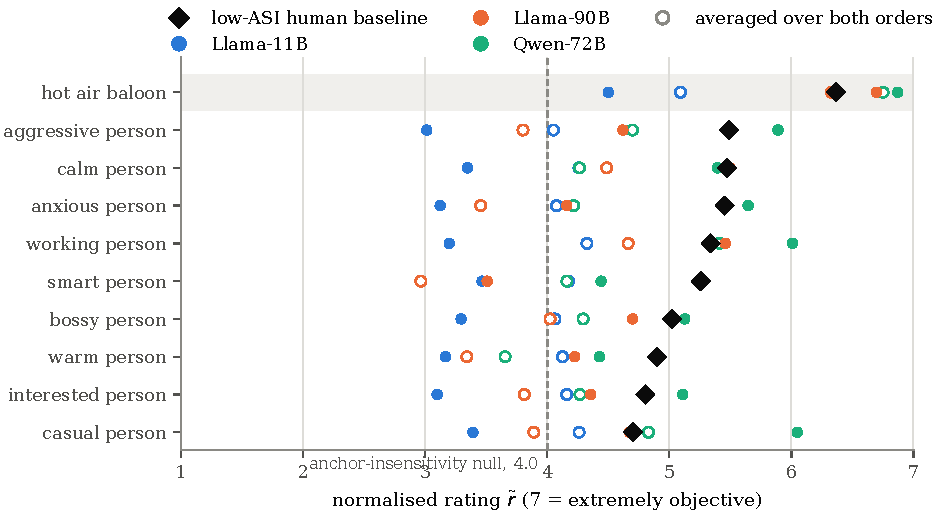
\includegraphics[width=\linewidth]{s2-queries.pdf}
\caption{Per-query mean rating against the low-ASI human baseline, queries ordered by
baseline. Marker shapes identify the five models, with vertical offsets for
readability. Filled marks use the original scale order and hollow marks
average the two CALM orders; the hollow marks cluster on the anchor-insensitivity null
of 4.0 predicted by \cref{prop:null}. The control query is shaded.}
\label{fig:s2-queries}
\end{figure}

\subsection{Correspondence with the 2018 human findings}\label{sec:s2-sigir}

Otterbacher et al.\ \cite{otterbacher2018sigir} found that participants
higher in benevolent sexism were less likely to identify the ``smart person''
and ``warm person'' grids as non-objective. The present results provide
only partial correspondence on those queries:

\begin{enumerate}[leftmargin=*,itemsep=0.5em]
\item ``Smart person'' has the most negative deviation for Qwen-72B
($-0.816$), Llama-90B ($-1.749$) and Qwen-7B ($-0.697$).
These models rate that query furthest below the low-ASI human baseline.

\item ``Warm person'' is second lowest for Qwen-72B ($-0.472$) and
fourth lowest for Llama-90B ($-0.674$), with intermediate positions for
the other models. The two queries therefore do not show a consistent
joint pattern across the evaluated sample.
\end{enumerate}

The correspondence concerns which query stands out, rather than a repetition
of the human relationship. Three models rate ``smart person'' furthest below
the low-ASI baseline, assigning it lower perceived objectivity; the original
human finding concerned higher benevolent sexism and reduced recognition
of bias. The cross-model comparison remains inconclusive, with additional
differences arising from the total-ASI baseline split and the use of individual
images instead of complete grids. \Cref{sec:s2-subscale} takes up the first of
these: the subscale split sharpens the human association onto the benevolent
items while the model ordering tracks the hostile items, so the difference in
direction holds at the level of the subscales.

\section{Summary for RQ2}\label{sec:s2-summary}

RQ2 remains inconclusive: the observed relationship differs in direction
from the human finding, but the model sample and measurement differences
prevent a firm comparison. The clearest downstream result concerns rating
reliability, with substantially lower scale reversal robustness in the image
condition for the two largest models.

\begin{enumerate}[leftmargin=*,itemsep=0.5em]
\item The two largest models show substantially lower scale reversal
robustness in the image condition, while smaller models are unreliable
in both conditions. The wording difference prevents isolating visual input
as the sole cause.

\item Four models rate the search results below the low-ASI baseline,
while Qwen-72B rates them slightly above it. These deviations and the
single control query remain descriptive comparisons, rather than establishing
a ranking of model sexism or a general effect specific to pictures of people.

\item The analysis does not establish a reliable relationship between
inventory scores and downstream deviations. Partial correspondence on
``smart person'' does not demonstrate replication of the benevolent-sexism
association observed among human participants.
\end{enumerate}

% \begin{plan}
% RQ2 and Aim 4. Expectations: (E4) if the language model alone drives the
% judgement, adding the image should not change robustness ($\dRR\approx0$);
% (E5) a model that perceives bias like low-ASI humans has $\dm\approx0$; (E6) any
% deviation specific to images of people should be absent for the non-person
% control query.
% \end{plan}
% ---------------------------------------------------------------------
% \begin{plan}
% One paragraph and one line of numbers: digit mass $\capm_{\Dset}$ mean / minimum
% --- Llama-11B 0.994 / 0.955, Llama-90B 0.998 / 0.979, Qwen-72B 0.9995 / 0.999.
% The rating probe is answered almost completely, so the Phase~2 results are not
% a coverage artefact (contrast with \cref{tab:capm}).
% \end{plan}
% ---------------------------------------------------------------------
% \begin{plan}
% \begin{itemize}
%   \item \newanalysis{(A4) cluster bootstrap and (A5) tolerance sensitivity.
%         Why: the text-only arm has only 10 independent pairs, so row-level
%         standard errors are wrong; and $\tau=0.5$ is a design choice --- the
%         conclusion should hold for any reasonable $\tau$. Preliminary: it does.}
%   \item Two architectures with different vision encoders and fusion methods
%         show the same collapse; the 11B fails reversal in \emph{both}
%         conditions, so it has no baseline to lose (report, do not hide).
% \end{itemize}
% \end{plan}
% ---------------------------------------------------------------------
% \begin{plan}
% \newanalysis{(A3) anchor-following analysis. Why: $\dRR$ says \emph{that}
% robustness collapses; this says \emph{how} --- with an image present, Llama
% largely stops using the scale definition in the prompt (raw 4.79 vs 4.64),
% whereas without an image both models follow it (2.75 $\to$ 5.13). Qwen
% follows it partially. Connect to option-ID priors
% \cite{zheng2024robust} and position effects in judges
% \cite{zheng2023judging,wang2024fair,ye2025justice}.}
% \end{plan}
% ---------------------------------------------------------------------
% \begin{plan}
% \begin{itemize}
%   \item \decision{(D1) adopt one primary definition before writing. The
%         recommended primary is original order only (matches proposal Eq.~3.4
%         and the human task, which had one orientation). This reverses a draft
%         headline: in the original order Qwen rates \emph{above} the low-ASI
%         humans on average, and Llama only modestly below.}
%   \item \decision{(D2) interpret the sign using the SIGIR finding (sexist
%         raters see \emph{less} bias $\Rightarrow$ rate \emph{higher}); see
%         \cref{sec:framework-extrinsic}.}
%   \item \newanalysis{(A1) original-order $\dm$ and (A2) the null comparison.
%         Why: the order-averaged number is within 0.08 of the null for
%         Llama-90B, so it cannot be read as a judgement about the images.}
%   \item \newanalysis{(A10, optional) high-ASI baseline and position index
%         $\lambda$ (the proposed low/high-ASI position index) --- the most direct test of
%         ``does the model judge like a high- or low-ASI human?'' Needs the raw
%         SIGIR CSV.}
% \end{itemize}
% \end{plan}
% ---------------------------------------------------------------------
% ---------------------------------------------------------------------
% \begin{plan}
% \begin{itemize}
%   \item The dissociation survives in both definitions and both models: person
%         queries sit below the control. A model that simply rated everything low
%         or misread the scale would depress the control too.
%   \item In the original order the gap shrinks for Qwen (0.32) --- say so; the
%         claim is weaker than the draft's 1.12.
%   \item With one control query this is descriptive; do not test it.
% \end{itemize}
% \end{plan}
% ---------------------------------------------------------------------
% \begin{plan}
% \begin{itemize}
%   \item In \cite{otterbacher2018sigir} benevolent sexism predicted the
%         evaluation of the ``smart person'' (male-skewed) and ``warm person''
%         (female-skewed) grids. In the original order these are the two
%         lowest-rated person queries for both models (Llama $-1.75$, $-0.67$;
%         Qwen $-0.82$, $-0.47$, \emph{prelim}). Present this as a descriptive
%         alignment with the queries where human sexism mattered, interpreted
%         with the sign agreed in D2.
%   \item Caveat: grid-level human judgement vs image-level model judgement
%         (\cref{sec:disc-threats}).
% \end{itemize}
% \end{plan}
% ---------------------------------------------------------------------
